\graphicspath{{./figures}}

\begin{figure}[!htb]
  \centering
  \begin{minipage}{.46\textwidth}
    \centering
    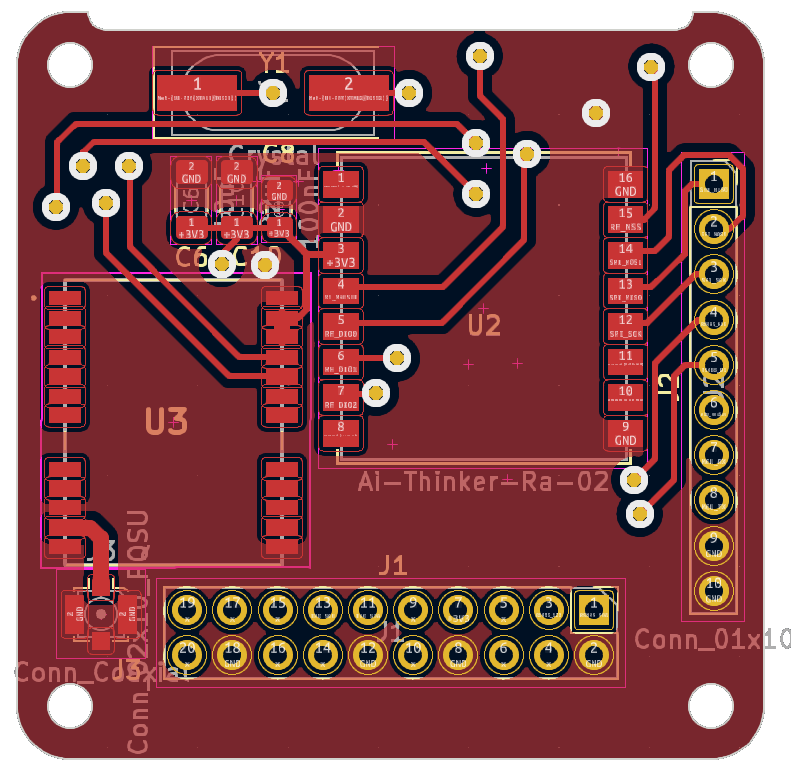
\includegraphics[width=.95\linewidth]{pqunit_pcb_design_front}
    \captionof{figure}{PocketQube Unit PCB Design (Front)}
    \label{fig:pqunit_pcb_design_front}
  \end{minipage}
  \begin{minipage}{.46\textwidth}
    \centering
    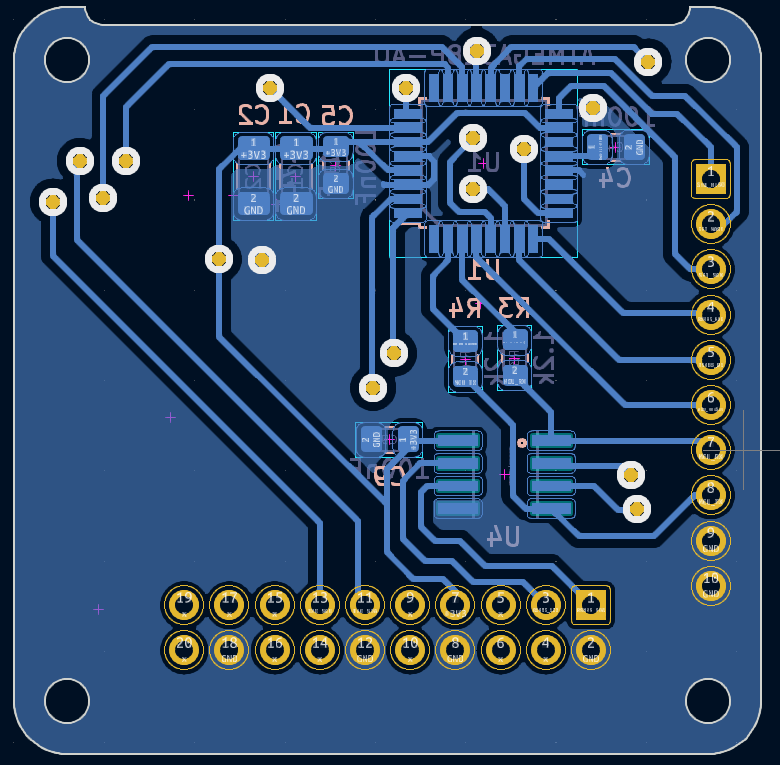
\includegraphics[width=.95\linewidth]{pqunit_pcb_design_back}
    \captionof{figure}{PocketQube Unit PCB Design (Back)}
    \label{fig:pqunit_pcb_design_back}
  \end{minipage}
  \end{figure}

\section{PocketQube Unit PCB}
\subsection{Circuit Design}
For the circuit design, the Arduino Nano schematic \cite{design-arduinoNano} was consulted as a reference. The pins needed to flash the MCU were exposed directly, instead of integrating a USB connection, for simplicity. The final schematic can be found in Appendix \ref{sec:appendix_pq_schematic}.

\subsubsection{RF and GPS Modules}
Since the RA-02 RF module has a u.FL connector onboard, no considerations need to be taken with respect to impedance matching. The ATGM332D GPS module, however, directly exposes its RF input via one of its SMD pins. The higher L1 GPS band operates around 1575.42 MHz, which is a wavelength of $\frac{3e8}{1575.42e6} = \SI{190}{mm}$. The ``critical length" (the length at which reflections can be ignored) is therefore around \SI{19}{mm}. If the module-antenna trace length is kept shorter than this, impedance matching will not be necessary.

\subsection{PCB Layout}
It was decided to use a 2-layer board, due to the low component count. Although impedance matching is not necessary for the GPS module, it is still desirable to control the trace impedance as much as possible. However, a 50-ohm trace on a 2-layer board is around $\SI{2.8}{mm}$ (determined using a microstrip impedance calculator). This is much larger than the GPS module pad sizes. The trace was therefore made as wide and as short as possible. The final PocketQube PCB is shown in Figures \ref{fig:pqunit_pcb_design_front} and \ref{fig:pqunit_pcb_design_back}.